\subsection{信用风险建模与评估 CR-5}


\subsubsection{CAMEL骆驼评级法}
\begin{itemize}
    \item 银行信贷分析师普遍采用 CAMEL 系统来评估银行信贷风险，该系统可被视为银行属性的核对清单，而这些属性被视为评估银行财务业绩的关键。
    \item 主要关注以下5个方面：
    \begin{itemize}
        \item C: Capital Adequacy 资本充足
        \item A: Asset Quality 资产质量
        \item M: Management 管理
        \item E: Earnings 盈利
        \item L: Liquidity 流动性
    \end{itemize}

\end{itemize}

\subsubsection{信用风险建模的要素}
\begin{itemize}
\item Probability of default（PD） 违约概率
    \begin{itemize}
    \item 反映违约发生的概率。
    \item PD的计算方法有很多种， 稍后会介绍多个模型
    \end{itemize}
\item Exposure at default（EAD） 风险敞口
    \begin{itemize}
    \item 反映实际暴露在信用风险中的资产价值。
    \item 【如果对方出现违约或无法履行合约，你可能会失去的钱。比如你有100元， 把钱全部借给你朋友， 那么你的预期敞口Expected Exposure（EE）=l00元。再比如， 你把20元存银行（假设这是无风险的）， 80元借给你朋友， 那么你的EE=80元】
    \end{itemize}
\item Loss given default（LGD） 违约损失率
    \begin{itemize}
    \item 指发生违约时扣除回收的部分所发生的损失率。
    \end{itemize}
\item Recovery Rate (RR)回收率：
    \begin{itemize}
    \item 在债券或贷款违约时，债权人能够收回的金额，占违约债务总额的百分比。
    \item  回收率与违约率负相关。
    \[LGD+RR=1\]

    \end{itemize}
\item Expected loss（EL）预期损失
    \begin{itemize}
    \item 指在未来一段时间（通常是一年）可能发生的平均损失。也就是损失的期望值。
\[\text{Expected loss（预期损失\%）} = \text{PD} \times \text{LGD}\]
\[\text{Expected loss（预期损失 \$）} = \text{PD} \times \text{LGD} \times \text{EAD}\]

\begin{note}{拓展： EL 的推导}

    一个资产未来有两种可能。一种是违约， 违约概率是PD， 如果违约， 因为有抵押品等还能回收RR，损失为1-RR。另外一种是不违约，收回全部资金， 损失为0。
$$EL=PD*(1-RR)+(1-PD)*0=PD * LGD$$

\end{note}

    \item tips: EL 是基于0 时刻位于未来风险的衡量。EL 本质上是未来的loss 。
    \end{itemize}
\end{itemize}



\subsubsection{Predicting Default in Credit Risk Models 违约概率的评估方法}
\begin{itemize}
    \item Judgmental approaches 判断法
    \begin{itemize}
        \item 也称作qualitative approaches 或expert systems，是最古老且最简单的信用风险评估方法。
        \item 完全基于信贷分析师对借款人基本质量和数量特征的专业判断。 
        \item 典型的分析方式是5C analysis：
        \begin{itemize}
            \item 1.character 品格：借款人的个性
            \item 2.capacity 能力： 基于现有的收入、支出和其他债务义务，评估借款人偿还贷款的能力。
            \item 3. capital 资本： 借款人面临风险的自有资本。
            \item 4. collateral 抵押品： 为偿付债务提供的担保品
            \item 5. conditions 条件：  描述商业环境状况和贷款特点（如利率）的一般条件。
        \end{itemize}
        \item 数据来源：
        \begin{itemize}
            \item 公开的财务报表publicly available financial statements : 资产负债表
            balance sheet、损益表income statement、现金流量表cash flow
            statement。
            \item 贷款申请中提交的商业计划business plan。
            \item 公司所在行业的数据。
            \item 公司所在地区的数据。
            \item 市场情况和总体经济前景等等。
        \end{itemize}
        \item 判断法的局限性
        \begin{itemize}
            \item 很难验证所获得结果的质量。
            \item 难以根据决策环境和可用信息的变化，更新评估过程的结构和实际结果。
            \item 很难检查可能影响单个借款人信用状况或整个信贷组合风险的情景。
            \item 可能会出现透明性和一致性问题，特别是在缺乏明确的实施和监控的情况下。
        \end{itemize}
    \end{itemize}

    
    

    \item Data-driven empirical models 数据驱动的经验模型
    \begin{itemize}
        \item 数据驱动经验模型根据贷款接受、拒绝、按协议支付和违约情况等历史数据构建模型。
        \item 适用于有历史数据的企业和消费者贷款。
        \item 数据来源包括银行内部数据库、信用评级机构和数据提供商。
        \item 使用统计学、机器学习和运筹学技术等， 进行大规模数据集， 识别复杂的非线性违约关系。
        \item 例如，芝麻信用评分；后面的信用评级（credit ratings）
        \item 优势：
        \begin{itemize}
            \item 流程提高了透明度（Transparency）和一致性（consistency）。
            \item 模型的基本结构及其预测能力可以通过实证检验。
            \item 可以进行假设检验、情景分析和压力测试。
            \item 可及时更新并定制化。 
        \end{itemize}
        \item 局限性：
        \begin{itemize}
            \item 依赖历史数据。
            \item 历史数据的静态和滞后性。
            \item 不能实时更新， 可能会忽略借款人最新状况。
        \end{itemize}
    \end{itemize}

    \item Financial models 金融模型
    

    金融模型采用规范性方法，基于规范的金融和经济理论建立。

    \begin{itemize}
        \item Structural models 结构模型 
            \begin{itemize}
            \item 结构模型假设企业的违约是一个内生过程， 由企业的结构特征（如资产价值和债务）决定。例如默顿模型（Merton model）。
            \end{itemize}

        \item Reduced form models简约模型
            \begin{itemize}
            \item 简约模型假设违约是随机事件，可能在任何时间发生，由外生随机变量——通常是泊松跳跃（Poisson jump）过程的变化——所驱动。这种模型使用债券和信用衍生品的市场数据作为了解企业信用风险结构的主要信息来源。
            \end{itemize}
        \end{itemize}
        \item Reduced-form models（简化模型）
    \end{itemize}

%【在这个章节中， 原版书还有其他内容， 笔记整理到了别处： 比如Capital Adequacy Ratio资本充足率， 在操作风险科目会有详细介绍。】

\subsection{Credit Scoring and Rating CR-6}

%【和FRM 一级中关于信用评级的知识有很大的相似度。如果一级这块知识学的比较扎实，这里可以少放些心思。】

\begin{itemize}
    \item 1. 基本概念
    \begin{itemize}
        \item 信用评分和信用评级，属于数据驱动的经验模型（Data-driven empirical models）。通过参考与借款人根据商定条款偿还债务的能力和意愿有关的所有可用信息，对借款人（债务人）的信用风险水平进行量化。
        
        \item Credit Scoring 信用评分
        \begin{itemize}
            \item 信用评分通常指为每个借款人提供数字信用评分的模型和系统。
            \item 信用评分是衡量借款人信用资质（Creditworthiness）和违约概率（Probability of default）的指标。
            \item 信用评分模型：输出一个反映借款人的信用资质和违约概率的分数。
            \item  信用评分通常仅供金融机构和企业客户内部使用。 
            \item  信用评分基于自动分析模型
            \item  例如， 芝麻信用分； FICO score。
        \end{itemize}
        \item Credit rating 信用评级
        \begin{itemize}
            \item 信用评级是以序数（ordinal）定性表示的风险评级， 例如A级、B级等。
            \item  每个风险等级都与根据经验估算的 违约概率相关联，该违约概率描述了所有被归入该等级的借款人。
            \item  信用评级通常用于公司贷款、债券发行和国家（例如主权信用评级），而且通常是公开的。
            \item 信用评级可能涉及分析性和判断性评估的结合，因此依赖于一个更加复杂和深入的过程。
        \end{itemize}
        \item 信用评级和信用评分是有序的，较高的评级意味着较低的信用风险，但评分或评级之间的差异与风险差异不成比例。
        \item 信用评分和评级系统的主要优势：
        \begin{itemize}
            \item 减少贷款评估过程中的主观性。
            \item 实现分析性的信用风险管理， 包括情景分析和压力测试。
            \item 通过对所有客户进行评估的共同框架，实现评估的一致性和透明性。
            \item 降低贷款评估所需的时间和成本。
        \end{itemize}
    \end{itemize}


    
\item 2. External ratings 外部评级
\begin{knowledgebox}{一级内容回顾}
    外部评级指的是外部第三方机构对金融机构的评级。

  %  【外部评级机构通常是独立的信用评级机构， 例如穆迪、标准普尔和惠誉等。】
    评级机构：根据特定标准对信用风险提供独立意见的组织。

    国际知名的三大评级机构：穆迪(Moody's)，标普(Standard and Poor's (S\&P))和惠誉(Fitch)

    评级机构对债券和货币市场工具使用不同的标准。
    
    \begin{itemize}
        \item 债券评级被称为长期评级。
        \item  货币市场工具的评级被称为短期评级。
        \end{itemize}

    惠誉的评级类别与标普一样。
    \begin{itemize}
        \item 投资级:BBB-(Baa3) 及以上

        \item 非投资级（投机级或垃圾债券）： BBB-（Baa3）以下。  
        【注意投资级和非投资级的划分界限】
        \end{itemize}
        

        \begin{center}
            {\renewcommand{\arraystretch}{1.5}  % 设置1.5倍行距
            \begin{tabular}{|l|l|l|p{7cm}|}  % 调整最后一列宽度为7cm，并将整个表格居中
            \hline
            \textbf{Category} & \textbf{Moody's} & \textbf{S\&P/ Fitch} & \textbf{Description} \\
            \hline
            \multirow{4}{*}{Investment grades} & Aaa & AAA & Highly recommended. Small risk of default. Stable investment. \\
            \cline{2-4}
            & Aa & AA & High quality investment. Slightly higher level of long-term risk. \\
            \cline{2-4}
            & A & A & High-medium quality investment. Vulnerable to economic changes. \\
            \cline{2-4}
            & Baa & BBB & Medium quality. Quite secure at present， with risk problems in long-term period. \\
            \hline
            \multirow{7}{*}{Speculative grades} & Ba & BB & Medium quality. Not well secured investment \\
            \cline{2-4}
            & B & B & Quite secure in present. Likely to default in the future. \\
            \cline{2-4}
            & Caa & CCC & Poor quality. High likelihood of default \\
            \cline{2-4}
            & Ca & CC & Highly speculative investment. Close to default. \\
            \cline{2-4}
            & & C & Low quality. High likelihood of default. Still paying at present. \\
            \cline{2-4}
            & C & D & In default. \\
            \hline
            \end{tabular}}
            \end{center}



    Rating agencies: organizations provide independent opinions on credit risk， based on specified criteria.

        \begin{itemize}
        \item Issue-specific credit ratings: specific obligations or instruments. 【债项评级】
        \item Issuer credit ratings: an issuer's general creditworthiness. 【发行人评级】
        \end{itemize}

    评级需同时考虑定量信息＋定性信息

    被评级公司给与评级公司fee 。这存在利益冲突， this fee arrangement has been
    criticized。
\end{knowledgebox}

\begin{itemize}
\item 两种评级方式: Through-the-Cycle versus Point-in-Time 


不论是外部评级还是接下来的内部评级，都可以使用这两种评级方式。 
    \begin{itemize}  
    \item Through-the-Cycle 全周期评级
        \begin{itemize}
        \item 周期评级反映一家公司数年内的平均信用度。考虑整体，不太受到整体经济状况起伏的过度影响。
        \item 评级比较稳定，监管机构倾向于使用 Through-the-Cycle 。
        \item 理论上， Through-the-Cycle 将低估经济周期下行的违约概率，而在经济周期上行时高估违约概率。
        \item 更新频率较低
        \item 适用于长期
        \end{itemize}

    \item  Point-in-Time 时间点评级
        \begin{itemize}
        \item  时间点评级旨在提供对未来违约概率的当前最佳估计。
        \item point-in-time ratings具有顺周期性，可能加剧经济波动.
        \item 评级波动较大，及时更新以反映新信息。
        \item 适用于短期。
        \end{itemize}
    \end{itemize}

    \item Development process 信用评分和评级模型的开发过程


信用评分和评级模型的开发是一个复杂和数据密集的过程，既需要分析人员的专业判断能力，也需要技术的先进性。

\begin{center}
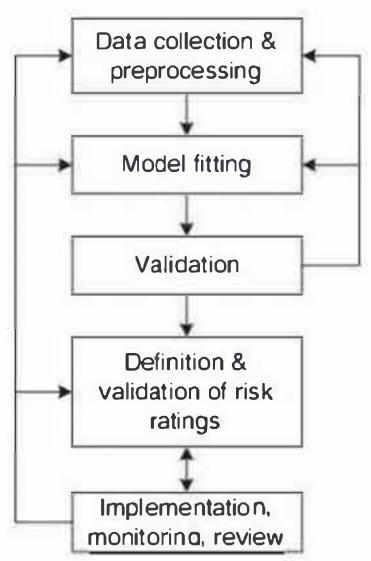
\includegraphics[width=0.3\textwidth]{images/019660e9-a588-71b6-ba51-02bd715bce7b_2_640_224_371_561_0.jpg}
\end{center}
\hspace*{3em} 


    \begin{itemize}
    \item a. Data Collection and Pre-processing 数据收集和预处理
        
    数据收集和预处理是信用评分/评级开发过程的首要步骤。
    
    收集违约/不违约的数据。
    
    数据预处理包括去除异常值、根据需要进行数据转换等。

    \item b. Model Fitting 模型拟合
        
确定最能描述(拟合)训练数据的模型参数 parameters。

比如线性回归模型，需要通过数据，找出参数 beta。

    \item c. Model Validation 模型验证


从模型拟合过程中得出的模型应使用与模型拟合所用样本不同的样本进行验证。

 Validation or holdout sample 验证样本或保留样本

使用样本外 (out-of-sample) 和时间外 (out-of-time) 数据进行回测（backtesting）， 来评估模型的预测性能。

        \item  d. Definition and Validation of Ratings 定义和验证评级

一旦信用评分模型通过验证，就需要把结果一一映射到不同的风险评级类别。

        \item e. Implementation 实施
        \begin{itemize}
            
            \item 最后阶段是将结果应用到信用评分/评级系统中，用于实时评估所有新申请贷款的信用风险。

            \item 经常进行监测和审查，并进行更新。
\end{itemize}
        \end{itemize}


\item    对信用评级机构的主要批评
        \begin{itemize}
        \item Lack of transparency and accountability， conflict of interest 缺乏透明度和问责制度，存在利益冲突：
        
        评级机构通常不公开披露如何进行其风险评级。且评级机构的收入依赖于被评级公司支付的费用。
        

        \item  Promoting Debt Explosion 促进债务增长：
        
        信用评分和评级提高了金融和信贷机构的风险估计能力， 从而使银行和其他信贷机构能够降低其风险溢价和债务融资成本。

        \item Poor Predictive Ability 预测能力不足：
        
        2007-2008 年全球信贷危机爆发， 评级机构未能预测到一些企业破产(如雷曼兄弟、安然等)引发了对评级机构评级预测能力的质疑。另外几项实证研究发现， 与金融机构内部开发的违约预测模型相比，评级机构的评级预测企业违约的能力较弱。

        \item Pro-cyclicality 顺周期性：
        
        在经济增长期间，评级过于乐观，在衰退时期过于悲观，因此显示出顺周期性的行为。 
\end{itemize}
\end{itemize}


\item 3. Internal ratings 内部评级
    \begin{itemize}
    \item Internal ratings vs. External ratings
        \begin{itemize}

        \item 外部评级： 通常只适用于已发行公开交易债务的公司。
        

        \item 内部评级：由银行等信贷机构使用，这些机构可以获得所需的历史数据，以开发和校准适合其特定信贷组合的模型。
        
        银行和其他金融机构开发自己的内部评级系统。
        \end{itemize}

    \item Altman's Z-Score 奥尔特曼Z评分模型
        \begin{itemize}

        \item  Altman 于 1968 年开发了后来被称为 Z-Score 的方法。是典型的内部评级模型。
        
        \item 利用一种称为判别分析的统计技术，从五个会计比率中预测违约情况：
        
        \[
        \mathrm{Z} = {1.21}{\mathrm{X}}_{1} + {1.4}{\mathrm{X}}_{2} + {3.3}{\mathrm{X}}_{3} + {0.6}{\mathrm{X}}_{4} + {0.999}{\mathrm{X}}_{5}
        \]
        
        \({\mathrm{X}}_{1}\) : 周转资金与总资产之比、=
        
        \({\mathrm{X}}_{2}\) : 留存收益与总资产之比
        
        \({\mathrm{X}}_{3}\) : 息税前利润与总资产之比
        
        \({\mathrm{X}}_{4}\) : 股本市值与总负债账面价值之比
        
        \({\mathrm{X}}_{5}\) : 销售额与总资产之比
        
        \item  判断:
        
        Z-score>3.0，不太可能违约
        
        \({2.7} < \mathrm{Z}\) -score \(< {3.0}\) ， 警惕
        
        \({1.8} < \mathrm{Z}\) -score \(< {2.7}\) ，有很大的违约可能性
        
        Z-score<1.8， 违约概率很高
        
        \item 【Z-score 只能得出违约与否的大概说明， 不能得出违约概率具体是多少】
        
        \item 【Z-Score 是基于 66 家公开交易的制造业公司样本估算的。该模型在样本外测试时表现相当准确。此外， 随着时间的推移， Z-Score 已经发展和扩展， 适用于非公开交易的制造业公司和非制造业行业。】
    \end{itemize}
\end{itemize}


    
    \item 4. Estimating Default Probabilities 估算违约概率
    
    违约概率 (probability of default， PD) 反映违约发生的概率。

    PD 的计算方法有很多种， FRM 一级考试主要掌握下面几种方法。
    \begin{itemize}
        \item （1）Unconditional and Conditional default probability 无条件和条件违约概率
        
        【注意题目的表达方法， 计算不同种类的概率】

            \begin{itemize}
            \item A. Cumulative Default Probability 累计违约概率
                \begin{itemize}
        
                \item  Cumulative PD：在一定时期内(例如，一年内、两年内、三年内)违约的概率
                
                \item Cumulative survival rate 累计生存概率 \(\left( {\mathrm{{SR}}}_{\mathrm{t}}^{\text{ cumulated }}\right)  = 1\) -cumulative PD
                \end{itemize}
           
        
            \item B. Unconditional default probability 无条件违约概率
                \begin{itemize}
                    \item 也称 Marginal Default Probability 边际违约概率
        
                    \item 指在某一特定时间段内，某一实体(如公司或债券发行人)发生违约的概率，而不考虑其他任何条件或前提。（后面的很多模型都是基于无条件违约概率）
                                        
                    \[
                    {\mathrm{{PD}}}_{\mathrm{k}}^{\text{ Uncond }} = {\mathrm{{PD}}}_{\mathrm{t} + \mathrm{k}}^{\text{ cumulated }} - {\mathrm{{PD}}}_{\mathrm{t}}^{\text{ cumulated }}
                    \]

                \end{itemize}
            \item C. Conditional default probability 条件违约概率
                \begin{itemize}
                    \item 条件违约概率是指在给定某些条件或前提下，某一实体在特定时间段内发生违约的概率。
        
                    \item 例如，存活(不违约)到第 \(\mathrm{n}\) 年，其在第 \(\mathrm{n} + 1\) 年违约的概率。
                    
                    \[
                    {\mathrm{{PD}}}_{\mathrm{t}，\mathrm{t} + \mathrm{k}}^{\text{ cond }} = \frac{{\mathrm{{PD}}}_{\mathrm{k}}^{\text{ Uncond }}}{{\mathrm{{SR}}}_{\mathrm{t}}^{\text{ cumulated }}}
                    \]
                \end{itemize}
        \end{itemize}
        
      
        
        \item （2） Historical Default Probabilities 历史违约概率
        
        根据历史数据计算出的违约概率，主要指评级机构的各类评级对应的违约概率。
        
\begin{itemize}


    \item Rating transitions 评级迁移矩阵【注意表头。下表 S\&P credit rating 由 1981-2000 年数据得到】
        
        Table 9.1 Average Cumulative Issuer-Weighted Default Rates (\%)， 1981-2020
        
        \begin{center}
        \adjustbox{max width=\textwidth}{
        \begin{tabular}{|c|c|c|c|c|c|c|c|c|}
        \hline
        \multirow{2}{*}{Rating} & \multicolumn{8}{|c|}{Time Horizon (years)} \\
        \cline{2-9}
         & 1 & 2 & 3 & 4 & 5 & 7 & 10 & 15 \\
        \cline{1-9}
        AAA & 0.00 & 0.03 & 0.13 & 0.24 & 0.34 & 0.51 & 0.70 & 0.90 \\
        \cline{1-9}
        AA & 0.02 & 0.06 & 0.11 & 0.21 & 0.30 & 0.49 & 0.70 & 0.99 \\
        \cline{1-9}
        A & 0.05 & 0.13 & 0.22 & 0.33 & 0.46 & 0.76 & 1.20 & 1.84 \\
        \cline{1-9}
        BBB & 0.16 & 0.43 & 0.75 & 1.14 & 1.54 & 2.27 & 3.24 & 4.54 \\
        \cline{1-9}
        BB & 0.63 & 1.93 & 3.46 & 4.99 & 6.43 & 8.89 & 11.64 & 14.65 \\
        \cline{1-9}
        B & 3.34 & 7.80 & 11.75 & 14.89 & 17.35 & 20.99 & 24.62 & 28.24 \\
        \cline{1-9}
        CCC/C & 28.30 & 38.33 & 43.42 & 46.36 & 48.58 & 50.75 & 52.76 & 54.76 \\
        \cline{1-9}
        \hline
        \end{tabular}
        }
        \end{center}
        
        \item 解读:
        
        例如，初始评级为 BBB 的债券在第一年的违约概率为 0.16\%，在 2 年内的累计违约概率为 0.43\%。
        
        计算特定年份的违约概率:评级为 BBB 的债券在第二年内(during the second year)的无条件违约概率为：
        
        \[0.27\%=0.43\% - 0.16\%\]
        
        条件违约概率 Conditional PD:
        \begin{itemize}
        
            \item 计算 CCC/C 评级公司的前两年不违约的条件下，第三年违约的概率：
        
            \[ \text{前两年不违约的概率} = {100}\%  - {38.33}\%  = {61.67}\%\]
            \[ \text{第三年违约的概率} = {43.42}\%  - {38.33}\%  = {5.09}\%\]
            \[ Conditional PD = {5.09\%}/{61.67\%} = {8.25}\% \]
        \end{itemize}

        
    \item 对于投资级债券，边际违约概率通常随时间递增。
        
    例如，初始評級為 A 的債券在第一年、第二年、第三年和第四年違約的概率分別為 {0.05}\% ，{0.08}\%  = ）{0.13}\%  - {0.05}\% ） ， 0.09\%=(0.22\%-0.13\%)，  0.11\%=(0.21\%-0.11\%)。
        
       
    这是因为债券发行人最初被认为信用可靠，时间流逝越久，其财务状况下降的可能性就越大。    
=
        
    \item 对于投机级债券: 边际违约概率可能随时间递减。
        
    例如，最初属于最低类别（CCC/C）的债券在第一年、第二年、第三年和第四年违约的概率分别为 28.3\%， 10.03\%， 5.09\%， and 2.94\%。
        
    这是因为，对于信用评级较差的债券来说，未来一两年可能至关重要。如果发行人能挺过这段时间，其财务状况很可能会有所改善。
    
    %【这与市场风险 “Chapter 7 Correlation Basics" 提到的相关概念是一致的】
        
        \item Default intensity model 违约强度模型
        
        Hazard Rate 风险率，也叫 default intensity 违约强度 (λ)，是短时间内（\(\Delta \mathrm{t}\) ）有条件违约概率的衡量标准 
        
        \(\lambda  * \bigtriangleup \mathrm{t}\) : 零时间到t时间之间没有违约的情况下， 时间 t 和 \(\mathrm{t} + \bigtriangleup \mathrm{t}\) 之间发生违约的概率。
        \[\text{ Cumulative }\mathrm{{PD}} = 1 - {\mathrm{e}}^{-\bar{\lambda }\mathrm{t}}\]
        \[\text{ Cumulative survival rate } = {\mathrm{e}}^{-\bar{\lambda }\mathrm{t}}\]
        \[\text{ Unconditional }\mathrm{{PD}} = {\mathrm{e}}^{-{\lambda }_{1} \times  {\mathrm{t}}_{1}} - {\mathrm{e}}^{-{\lambda }_{2} \times  {\mathrm{t}}_{2}}\]
        
        \(\bar{\lambda }\) 是时间零点至时间点t之间的平均风险率。 
        
        例如：假设每年的风险率是恒定的 1.5\%。
        
        第一年年底发生违约的概率是 \(1 - {\mathrm{e}}^{-{0.015} \times  1} = {0.0149}\) 。
        
        到第二年年底发生违约的概率是 \(1 - {\mathrm{e}}^{-{0.015} \times  2} = {0.0296}\)
        
        在第三年、第四年和第五年结束时发生违约的概率分别为0.0440， 0.0582， 和0.0723
        
        
         第四年的无条件违约概率为\({0.0582} - {0.0440} = {0.0142}\) 
        
         在没有提前违约的条件下，第四年违约的概率为 0.0142/(1- 0.0440) = 0.0149
        
        \item Recovery Rates 回收率
        

        \begin{table}[htbp]
            \centering
            \caption{1983 到 2021 不同公司债券种类的回收率}
            \adjustbox{max width=\textwidth}{
                \begin{tabular}{|c|c|}
                \hline
                Class & Average Recovery Rate (\%) \\
                \cline{1-2}
                1st lien bond & 54.6 \\
                \cline{1-2}
                2nd lien bond & 44.3 \\
                \cline{1-2}
                Senior unsecured bond & 38.0 \\
                \cline{1-2}
                Senior subordinated bond & 31.0 \\
                \cline{1-2}
                Subordinated bond & 32.1 \\
                \cline{1-2}
                Junior subordinated bond & 22.3 \\
                \cline{1-2}
                \hline
                \end{tabular}
            }
        \end{table}
        
        【债券种类稍微了解即可——公司破产清算时的求偿顺序为: First Lien Loan优先级最高，回收率因此最高；后面依次递减， Junior Subordinated回收率最低。】 
        
        2007-2008 年危机的教训：抵押贷款回收率与抵押贷款违约率呈负相关。公司债券也存在类似的负相关关系。
        
    【经济疲软时，借出方不仅面临违约率上升的更大风险，还会由于回收率低而遭受更大的损失。】

    \end{itemize}
\end{itemize}

\end{itemize}


\subsection{计算违约概率 CR-9}

\subsubsection{信用利差计算违约概率}



1. 基本概念

\begin{itemize}
\item 粗略地说，信用利差（credit spread）可视为平均损失率。

\[ \text{credit spread} \approx  \mathrm{{EL}}\left( \% \right)  = \mathrm{{PD}} * \mathrm{{LGD}} = \mathrm{{HazardRate}} * \left( {1 - \mathrm{{RR}}}\right)\]
\[\rightarrow   \text{Hazard Rate} \left( \lambda \right)  = \text{credit spread} /\left( {1 - \mathrm{{RR}}}\right)\]

\begin{itemize}
    \item Recover Rate（RR）  回收率
\end{itemize}

 \item 原版书例子: 假设 3 年期、5 年期和 10 年期的 CDS 息差分别为 50、60 和 100 个基点，预期回收率为 60\%。
 \begin{itemize}

    \item 三年的平均风险率约为 0.005/(1 - 0.6) \(= {0.0125}\) 

    \item 五年的平均风险率约为 0.006/(1 - 0.6) \(= {0.015}\) 

    \item 十年的平均风险率约为 \({0.01}/\left( {1 - {0.6}}\right)  =\) 0.025 .

    \item 第 3 年至第 5 年的平均风险率为 (5* 0.015 - 3*0.0125)/2 = 0.01875 .

    \item 第 5 年至第 10 年的平均风险率为 \(({10} * {0.025} - 5\)  \(* {0.015})/5 = {0.035}\) .

\end{itemize}

\end{itemize}


2. 信用利差的种类

\begin{itemize}
\item A. CDS(Credit credit swap) spread 信用违约互换利差


\begin{figure}[htbp]
    \centering
    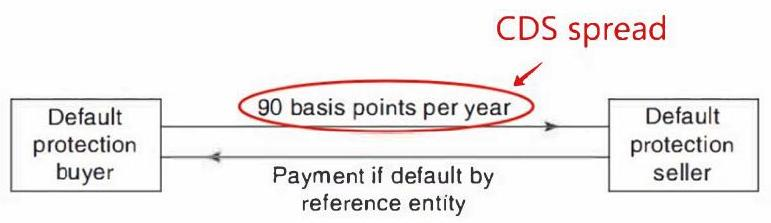
\includegraphics[width=0.6\textwidth]{images/019660e9-a588-71b6-ba51-02bd715bce7b_8_435_1735_771_223_0.jpg}
    \caption{信用违约互换（Credit default swap）}
    \label{fig:cds}
\end{figure}

\begin{itemize}
    \item CDS spread 是购买信用违约互换时需支付的保险费 premium。

    \item 反映了特定债务发行人的违约风险。发行人(reference entity)违约风险较高，CDS spread 越高，反之亦然。

\end{itemize}

\item B. Bond yield spread 债券收益率利差


\begin{itemize}
    \item 债券收益率利差是指公司债券收益率与类似无风险债券收益率之差。
    \item 反映了特定债务发行人的违约风险。发行人违约风险较高，债券收益率利差越高，反之亦然。

    \item 通常:债券收益率利差=YTM \({}_{\text{ 公司债 }} -\) YTM \({}_{\text{ 国债 }}\)
    

    \item CDS-债券基差（CDS-bond Basis）是  CDS 利差超出债券收益率利差的部分。
\[CDS-Bond Basis= CDS Spread - Bond Yield Spread\]

\item 如果是同一个实体 (债券发行人)， 风险情况一定， 那么 CDS Spread 应该等于 Bond Yield Spread， 即 CDS-Bond Basis 应接近零， 但实际上往往偏离零。

 CDS-Bond Basis 偏离零的原因:
 
 %【原版书这里给了原因和影响结果，但是没有给出具体原因， 所以这里原因的解释， 稍作了解即可。】
\begin{itemize}

\item Negative direction， 即 CDS Spread < Bond Yield Spread

CDS 存在交易对手违约风险。【CDS 的卖方违约风险大(即 CDS 的卖方不赔付)→ CDS 不值钱 → CDS Spread↓ 】


CDS 的偿付未包括交付债券的累计利息（interest）。【CDS 少考虑了一部分 “好处 accrued interest” \(\rightarrow\) CDS 不值钱 \(\rightarrow\) CDS Spread \(\downarrow\) 】

 \item Positive direction， 即 CDS Spread > Bond Yield Spread

 There is a cheapest-to-deliver bond option in a CDS. 【这个 option 对于 CDS 是好的 \(\rightarrow\) CDS 更值钱 \(\rightarrow\) CDS Spread [1]

 The restructuring clause(重组条款) in a CDS contract may lead to a payoff when there is no default. 【restructuring clause 对于 CDS 是好的 \(\rightarrow\) CDS 更值钱 \(\rightarrow\) CDS Spread \(\uparrow\) 】

重组条款(Restructuring Clause)是 CDS 合约中的一项条款， 规定如果参考实体的债务发生某种形式的重组 (如修改偿还条件、 延长债务期限或降低利率等)，即使参考实体没有违约， CDS 买方也可以获得赔付。

\item 可能 Negative direction， 也可能 Positive direction

\begin{itemize}
\item 债券的售价可能与面值相差很大。

高于面值的债券价格往往会产生负基差。

低于面值的债券价格往往会产生正基差

\item 【无风险利率的选择不同】

债券收益率利差可能是相对于无风险参考利率计算的，而这个参考利率并不是市场上使用的利率。
\end{itemize}

\end{itemize}

\item 若 CDS-Bond Basis \(\neq  0\) ，即 CDS Spread \(\neq\) Bond Yield Spread
\begin{itemize}

    \item CDS Spread \(>\) Bond Yield Spread \(\rightarrow\) 卖出 CDS(收 CDS Spread)，做空债券 (支出 coupon)

    \item CDS Spread \(<\) Bond Yield Spread \(\rightarrow\) 买入 CDS(支出 CDS Spread)，做多债券(收 coupon)
\end{itemize}

 \item 市场动荡前后的基差趋势:

【CDS-Bond Basis 偏离零的情况】
\begin{itemize}

    \item 次贷危机前: the basis tended to be positive.

    \item 次贷危机期间: 基差有时非常负，但由于流动性短缺和其他考虑， 金融机构难以在债券和 CDS 之间进行套利。

    \item 次贷危机后: CDS-Bond Basis 通常较小且为负。
\end{itemize}
\end{itemize}

 \item C. Asset swap spread

\begin{itemize}
\item 资产互换（Asset swaps）为信贷市场的交易者提供了一个方便的参考点，因为它能直接估算出债券收益率超过浮动参考利率的部分。【简单了解】

\end{itemize}

\begin{center}
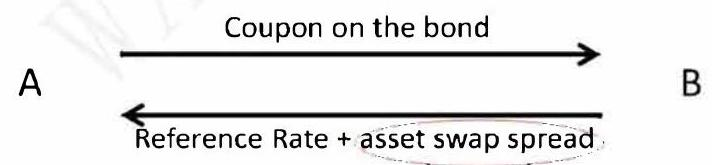
\includegraphics[width=0.6\textwidth]{images/019660e9-a588-71b6-ba51-02bd715bce7b_10_460_1396_712_165_0.jpg}
\end{center}
\hspace*{3em} 

小结:
\begin{itemize}

    \item 使用bond yield spreads和 asset swap spreads 计算 hazard rate ，需要满足一定的前提条件: 标的债券以接近其面值的价格出售。

    \item 如果不是 par bond，需要可以采用其他方式求得 hazard rate。%【具体怎么求， 不在考纲范围内。这里就不做介绍】
\end{itemize}



3. Comparing default probabilities 比较违约概率

\begin{itemize}
\item 比较从历史数据(来自标普)计算的累计违约概率与从信用利差(来自美林 Merrill Lynch)计算的累计违约概率

\begin{table}[htbp]
    \renewcommand{\arraystretch}{1.3} % 调整行高，1.3 可根据需要修改

    \centering
    \caption{累计违约概率与信用利差对比}
    \adjustbox{max width=\textwidth}{
        \begin{tabular}{|c|c|c|}
        \hline
        Rating & Cumulative 7-Year Default Probabilities (\%)，1981-2020 & 7-Year Credit Spread (bp) 1996-2007 \\
        \cline{1-3}
        AA & 0.51 & 35.74 \\
        \cline{1-3}
        AA & 0.49 & 43.67 \\
        \cline{1-3}
        A & 0.76 & 68.68 \\
        \cline{1-3}
        BBB & 2.27 & 127.53 \\
        \cline{1-3}
        BB & 8.89 & 280.28 \\
        \cline{1-3}
        B & 20.99 & 481.04 \\
        \cline{1-3}
        CCC/C & 50.75 & 1,103.70 \\
        \cline{1-3}
        \hline
        \end{tabular}
    }
\end{table}

 
\end{itemize}
\item 例如: A 评级的累计违约=0.76\%，求得 hazard rate
\[ \text{Cumulative} \mathrm{{PD}} = 1 - {\mathrm{e}}^{-\lambda \mathrm{t}} \rightarrow  {0.76}\%  = 1 - {\mathrm{e}}^{-\lambda  * 7} \rightarrow   \rightarrow  \lambda  = {0.1090}\%\]

\item A 评级的 CS=0.6868\%(The recovery rate is assumed to be 40\%)， 求得 hazard rate
\[\lambda  = {0.6868}\% /\left( {1 - {40}\% }\right)  = {1.1447}\%\]

\begin{table}[H]
    \renewcommand{\arraystretch}{1.3} % 可选：增加行高
    \centering
    \caption{平均七年违约强度（Hazard Rate）}
    \adjustbox{max width=\textwidth}{
        \begin{tabular}{|c|c|c|c|}
        \hline
        Rating & Rate from Default Probabilities (\%) & Rate Implied by Credit Spreads (\%) & Difference \\
        \cline{1-4}
        AAA & 0.073 & 0.596 & 0.523 \\
        \cline{1-4}
        AA & 0.070 & 0.728 & 0.658 \\
        \cline{1-4}
        A & 0.109 & 1.145 & 1.036 \\
        \cline{1-4}
        BBB & 0.328 & 2.126 & 1.798 \\
        \cline{1-4}
        BB & 1.330 & 4.671 & 3.341 \\
        \cline{1-4}
        B & 3.366 & 8.017 & 4.651 \\
        \cline{1-4}
        CCC/C & 10.118 & 18.395 & 8.207 \\
        \cline{1-4}
        \(\%\) per annum.&&&\\
        \cline{1-4}
        \hline
        \end{tabular}
    }
\end{table}


\item 由 CS 计算的违约概率大于历史数据(期限更长 1981-2020)得出的违约概率。

\item 随着信用质量下降，两种违约率之间的差异也在增加。Reason for the Difference:
\begin{itemize}

\item Corporate bonds are relatively illiquid. 【债券的流动性不好，因此收益率比较高来补偿流动性风险。然而， 这只能解释 difference 的一小部分，大约 25 个基点。】

\item the subjective default probabilities 主观违约概率 of bond traders are much higher 【债券交易员对违约概率的主观判断可能要更高】

\item bonds do not default independently of each other. 【债券违约与否并不是独立的 \(\rightarrow\) systematic risk \(\rbrack\)

* Credit contagion 信用传染: 市场经济好， 降低了所有公司的违约概率，而市场条件不好，则增加了所有公司的违约概率

\item nonsystematic (or idiosyncratic) risk

每只债券都伴随有非系统性风险， 这种风险难以通过持有少数债券来有效分散， 需要补偿。【债券一个典型的特征是: 收益少 (只有利息)，但是损失比较大(不仅利息也可能本金)】


\end{itemize}

\end{itemize}


\subsubsection{股价计算违约概率}

\begin{itemize}
\item 1. Merton model 莫顿模型

\begin{itemize}
\item 一种结构化模型（ Structural model ）。与 BSM 模型有着千丝万缕的关系。【根据公司股票的实时价格得出公司的违约概率】

%\item it depends on the structure of the company's balance sheet-its assets， liabilities， and equity. It also can be called a company-value model because the key variable is the asset value of the company.
\item 它取决于公司资产负债表的结构——资产、负债和权益。由于关键变量是公司的资产价值，因此也可称为公司价值模型。

\item 基于以下假设: 
\begin{itemize}

    \item a. 债务负债是在 T 时间到期的零息债券。

    \item b. 违约概率是这一结构模型的内生因素。

    \item c. 公司的资产可自由交易。
\end{itemize}

\item 逻辑:【公司资产asset=负债+股东权益】

 假设某公司的资产价值 V，同时公司向债权人发行了面值为 \(\mathrm{K} = {100}\) ，期限为 1 年的零息债券， 到期一次性偿还本金。一年后债券到期日， 债券持有人和股权持有人的价值情况:

\begin{center}
\adjustbox{max width=\textwidth}{
\begin{tabular}{|c|c|c|c|}
\hline
一年后 & 资产价值 \(\left( {\mathrm{V}}_{1}\right)\) & 债券价值 \(\left( {\mathrm{B}}_{1}\right)\) & 股东权益 \(\left( {\mathrm{S}}_{1}\right)\) \\
\cline{1-4}
情况 1 & \({\mathrm{V}}_{1} = {300} > \mathrm{K}\) & \({\mathrm{B}}_{1} = \mathrm{K} = {100}\) & \({\mathrm{S}}_{1} = {200} = {\mathrm{V}}_{1} - \mathrm{K}\) \\
\cline{1-4}
情况 2 & \({\mathrm{V}}_{1} = {100} = \mathrm{K}\) & \({\mathrm{B}}_{1} = \mathrm{K} = {100}\) & \({\mathrm{S}}_{1} = 0 = {\mathrm{V}}_{1} - \mathrm{K}\) \\
\cline{1-4}
情况 3 & \({\mathrm{V}}_{1} = {80} < \mathrm{K}\) & \({\mathrm{B}}_{1} = {\mathrm{V}}_{1} = {80}\) & \({\mathrm{S}}_{1} = 0\) \\
\cline{1-4}
一般情况 & \({\mathrm{V}}_{1} ={\mathrm{B}}_{1} + \mathrm{S_1}\) & \({\mathrm{B}}_{1} = \operatorname{Min}\left( {\mathrm{K},{\mathrm{V}}_{1}}\right)= K-Max(K-V_1,0) \) & \({\mathrm{S}}_{1} = \operatorname{Max}\left( {{\mathrm{V}}_{1} - \mathrm{K},0}\right)\) \\
\cline{1-4}
\hline
\end{tabular}
}
\end{center}

\item 结论:
\begin{itemize}
    
\item 对于股东来说:【持有公司股票，等同于持有一个标的资产是公司资产， 执行价格是K的欧式看涨期权 】
\[\text{ 股东权益 }\left( {\mathrm{E}}_{0}\right)  = \mathrm{{VN}}\left( {\mathrm{d}}_{1}\right)  - {\mathrm{{Ke}}}^{-\mathrm{{rT}}}\mathrm{N}\left( {\mathrm{d}}_{2}\right)\]
\[{d}_{1} = \frac{\ln \left( \frac{v}{K}\right)  + \left( {r + \frac{{\sigma }^{2}}{2}}\right) T}{\sigma \sqrt{T}},{d}_{2} = \frac{\ln \left( \frac{v}{K}\right)  + \left( {r - \frac{{\sigma }^{2}}{2}}\right) T}{\sigma \sqrt{T}}\]
\[{\mathrm{d}}_{2} = {\mathrm{d}}_{1} - \sigma \sqrt{\mathrm{T}}\]
\[\Phi :\text{Volatility of assets (assumed constant)}\]

\item 对于债权人来说【千万记得，债务价值不是 put 价值】

 \({\mathrm{B}}_{1} = \operatorname{Min}\left( {\mathrm{K},{\mathrm{V}}_{1}}\right)  = \mathrm{K} - \operatorname{Max}\left( {\mathrm{K} - {\mathrm{V}}_{1},0}\right)  = \mathrm{K} -\) put option

* Value of risky debt = value of risk-free debt - value of a put option

 持有公司的债务， 等同于持有一种无风险债券 (面值为 K)， 并同时卖出一个欧式看跌期权(标的资产是公司资产，执行价格是 \(\mathrm{K}\) )

 \({\mathrm{B}}_{1} = {\mathrm{V}}_{1} - {\mathrm{E}}_{1} = {\mathrm{V}}_{1} - \operatorname{Max}\left( {{\mathrm{V}}_{1} - \mathrm{K},0}\right)  = {\mathrm{V}}_{1}\) -call

 持有公司的债务， 等同于持有公司资产， 同时卖出一个欧式看涨期权

\item 风险中性违约概率 Risk-neutral probability of default=看涨期权不行权的概率= \(1 - \mathrm{N}\left( {\mathrm{d}}_{2}\right)\) 

回顾 BSM: 期权的价值

\[\mathrm{{Call}} = {\mathrm{S}}_{0}\mathrm{\;N}\left( {\mathrm{\;d}}_{1}\right)  - {\mathrm{{Xe}}}^{-\mathrm{{rT}}}\mathrm{N}\left( {\mathrm{d}}_{2}\right)\]
\[\text{ Put } = X{e}^{-{rT}}N\left( {-{d}_{2}}\right)  - {S}_{0}N\left( {-{d}_{1}}\right)\]
\[\mathrm{N}\left( {\mathrm{d}}_{1}\right)  + \mathrm{N}\left( {-{\mathrm{d}}_{1}}\right)  = 1\]
\[{d}_{1} = \frac{\ln \left( \frac{{S}_{0}}{x}\right)  + \left( {r + \frac{{\sigma }^{2}}{2}}\right) T}{\sigma \sqrt{T}}\]
\[{d}_{2} = \frac{\ln \left( \frac{{S}_{0}}{x}\right)  + \left( {r - \frac{{\sigma }^{2}}{2}}\right) T}{\sigma \sqrt{T}}\]
\[{\mathrm{d}}_{2} = {\mathrm{d}}_{1} - \sigma \sqrt{\mathrm{T}}\]

N(X): Standard normal cumulative distribution function.

\(\mathrm{N}\left( {\mathrm{d}}_{1}\right)\) : Delta of call option

\(\mathrm{N}\left( {\mathrm{d}}_{2}\right)\) : Risk-neutral probability of call exercise 行权概率

\item Distance to default (DD) 违约距离

违约距离是指在未来 T 年触发违约所需的，资产价格变化的标准差数量。

\[
{DD} = {d}_{2} = \frac{\ln \left( \frac{V}{K}\right)  + \left( {r - \frac{{\sigma }^{2}}{2}}\right) T}{\sigma \sqrt{T}} \approx  \frac{\ln \left( V\right)  - \ln \left( K\right) }{\sigma }
\]

违约距离越小，公司更有可能违约。

通过计算 \(\mathrm{{DD}}\) ，通过查标准正态分布表即可得违约概率。

另外， 当有几个备选可投资的公司， 无需精确算出每个公司的违约概率， 只需要知道几个公司的 DD 大小即可， DD 越大越安全。

\item Firm value(V) 和 Volatility of firm value \(\left( \sigma \right)\)

计算违约概率时，需要知道资产价值 \(\mathrm{V}\) 和资产价值的波动率，可以通过下面等式求解。本身的求解过程并不重要(计算过程很复杂)， 结果也不重要。关键掌握这一点一一Volatility of firm value 和 the volatility of firm 即使未知， 也依然可以利用 Merton model 求出违约概率。即 Volatility of firm value 和 the volatility of firm 未知， 不是 Merton model 的缺陷。

联立下面两个方程，可求出 \(\mathrm{V}\) 和 \(\sigma\) :

\[\text{ delta } = \mathrm{N}\left( {\mathrm{d}}_{1}\right)  = \frac{\text{ 期权价格的变化 }}{\text{ 标的资产价格的变化 }} = \frac{{\sigma }_{\mathrm{E}} \times  {\mathrm{E}}_{0}}{{\sigma }_{\mathrm{V}} \times  {\mathrm{V}}_{0}} \rightarrow  {\sigma }_{\mathrm{E}} \times  {\mathrm{E}}_{0}\]
\[= \mathrm{N}\left( {\mathrm{d}}_{1}\right)  \times  {\sigma }_{\mathrm{V}} \times  {\mathrm{V}}_{0}\]
\[\left. \begin{array}{l} {\mathrm{E}}_{0} = \mathrm{{VN}}\left( {\mathrm{d}}_{1}\right)  - {\mathrm{{Ke}}}^{-\mathrm{{rT}}}\mathrm{N}\left( {\mathrm{d}}_{2}\right) \\  {\sigma }_{\mathrm{E}} \times  {\mathrm{E}}_{0} = \mathrm{N}\left( {\mathrm{d}}_{1}\right)  \times  {\sigma }_{\mathrm{V}} \times  {\mathrm{V}}_{0} \end{array}\right\}   \rightarrow  \text{ 可得: }\mathrm{V}\text{ 和 }\sigma\]
\end{itemize}

\end{itemize}


\item 2. Merton model 的扩展模型， 有很多种形式， 例如:
什么情况下算违约， 即资产价值小于多少算违约: a default occurs whenever the value of the assets falls below a barrier level. 【当资产价值跌破某个障碍水平， 认为就会发生违约。】
%这里感觉可以出一个对比的表格， 比较不同模型之间的差异
最基本的莫顿模型:barrier level 是债务价值。扩展模型:barrier level 可以是其他设定的情况

Another allows payments on debt instruments to be required at more than one time.

最基本的莫顿模型:假设公司的所有债务只有一个到期时间(即所有债务一次性到期)。

扩展模型:实际上，公司的债务发生在多个时间点。例如，公司可能有分期偿还的债务或本身有不同到期日的债券。

 下面的 Moody's-KMV model and the Kamakura model 也是其中的一个扩展模型

 \item 3. Moody's-KMV model and the Kamakura model【原版书这里介绍的甚少】
\begin{itemize}

    \item 都是基于默顿模型 Merton model 的框架，用于估计公司的违约概率。

    \item Moody's-KMV 模型:

由 Moody's Analytics 旗下的 KMV 开发， 更加专注于利用市场数据和公司财务数据来估计违约概率。它将 Merton 模型的理论应用于实际市场数据中， 提供了一种量化的风险评估工具。


\item Kamakura 模型:

由 Kamakura 公司开发，同样也是基于公司财务数据和市场数据来计算违约概率的模型。在具体的数学公式和模型参数上有所不同， 但目标和方法与 Moody's-KMV 模型类似。

\item Moody's KMV and Kamakura provide services to transform Merton's model default probabilities into real-world default probabilities.
\end{itemize}

\item 4. Real-World vs. Risk-Neutral Default Probabilities

\begin{itemize}
\item In a risk-neutral world， the expected growth rate of the value of the company's assets is the risk-free rate.

\item In the real world， the growth rate of the company's assets is usually higher than this (reflecting a risk premium demanded by the market).

\item Risk-Neutral Default Probabilities 风险中性违约概率

\item Real-World Default Probabilities 真实世界违约概率

也叫 physical default probabilities
\end{itemize}
\begin{table}[htbp]
    \renewcommand{\arraystretch}{1.3} % 调整行高
    \centering
    \caption{风险中性违约概率与现实世界违约概率的比较}
    \adjustbox{max width=\textwidth}{
        \begin{tabular}{|c|p{6cm}|p{6cm}|}
        \hline
        \phantom{X} & 风险中性违约概率 & 现实世界违约概率 \\
        \cline{1-3}
        含义 & 在风险中性世界中计算的公司违约的概率。假设投资者对风险无偏好，公司资产的预期增长率等于无风险利率。 & 在现实经济环境中，公司实际发生违约的概率。考虑了市场对风险的态度，因此反映了投资者预期的公司资产增长率，该增长率通常高于无风险利率，因为包括了风险溢价。 \\
        \cline{1-3}
        资产的增长率 & 无风险利率 & 高于无风险利率（反映了风险溢价） \\
        \cline{1-3}
        数据 & 基于信用利差 & 基于历史数据（例如评级机构） \\
        \cline{1-3}
        适用场景 & 适用于估值，因为它们更接近无偏的市场定价。 & 适用于情景分析，因为更能反映实际经济条件下的违约风险。 \\
        \cline{1-3}
        模型 & Merton 模型 & Moody's-KMV 和 Kamakura 模型 \\
        \cline{1-3}
        \multicolumn{3}{|c|}{风险中性违约概率高于现实世界违约概率。} \\
        \cline{1-3}
        \hline
        \end{tabular}
    }
\end{table}

\end{itemize}


\subsection{Retail Credit Risk Management CR-7}


1. 基本概念

\begin{itemize}
\item 零售银行 retail banking 主要接受消费者和小企业的存款以及向其提供贷款。

\item 贷款形式包括:

 房屋抵押贷款 Home mortgages、房屋产权信贷额度 Home equity loans(HELOCs)、分期付款贷款 Installment loans(涵盖汽车、信用卡等)、小企业贷款 Small Business Loans (SBL)。

\item 主要风险:

 信用风险 credit risk

 运营风险：与业务运营相关的日常风险。

 业务风险：与新产品或趋势相关的战略风险，以及与利率变化时抵押贷款量等措施相关的数量风险。
 
 声誉风险：银行在客户和监管机构中的声誉。
 
 利率风险：银行为其资产和负债提供特定利率，利率随市场变化而变化。
\begin{comment}
Operational risks: day-to-day risks associated with running the business.

Business risks: strategic risks associated with new products or trends and volume risks associated with measures like mortgage volume when rates change.

Reputation risks: the bank's reputation with customers and regulators.

Interest rate risks: the bank provides specific interest rates to its assets and liabilities and rates change in the marketplace.
\end{comment}

 资产估值风险Asset valuation risk ：与资产、负债和抵押品类估值相关的市场风险

\item 零售风险为具有以下特征的同质化组合 homogeneous portfolios:

 A large number of small， low-value loans 大量的小额、低价值贷款With either a consumer or business focus Where the incremental risk of any single exposure is small 增量风险较小

\end{itemize}


2. Retail credit risk vs. Corporate credit risk

\begin{itemize}
\item Retail credit risk 零售信用风险
\end{itemize}

\begin{itemize}
\item 即使单个客户违约，影响也很小

\item Expected loss can be treated like other costs of doing business and can be built into the price charged. 【预期损失可以体现在产品定价中】

\item Corporate credit risk 公司信用风险
\begin{itemize}

    \item 单一名称的大额风险敞口Large exposures to single name;

    \item Concentrations of exposures.

    \item 以信贷损失上升到某种意外水平的风险为主。 Dominated by the risk that credit losses will rise to some unexpected level.
\end{itemize}

\end{itemize}

3.The Dark Side 阴暗面 of Retail Credit Risk

【正常情况下， 零售银行风险对于银行来说并不会带来太大影响， 但有些时候却会带来很大问题】

4 个原因:

\begin{itemize}
\item 并非所有创新的零售信贷产品都能与足够的历史损失数据相关联，从而使其风险评估变得可靠。【缺乏足够的历史损失数据， 风险难以评估】
\end{itemize}

\begin{itemize}
\item 在经济环境急剧变化的影响下，特别是在风险因素同时恶化的情况下（即所谓的完美风暴情景），即使是广为人知的零售信贷产品也可能开始出现意想不到的行为。 Even well-understood retail credit products might begin to behave in an unexpected fashion under the influence of a sharp change in the economic environment， particularly if risk factors all get worse at the same time (the so-called perfect storm scenario). 【未预料到的经济环境急剧变化】
\end{itemize}

\begin{itemize}
\item 消费者违约（或不违约）的倾向是一个复杂的社会和法律体系的产物，而这个体系又在不断变化。 The tendency of consumers to default (or not) is a product of a complex social and legal system that continually changes. 【消费者违约行为的复杂性: 消费者违约行为受到复杂的社会和法律制度的影响， 并且这些制度不断变化。】
\end{itemize}

\begin{itemize}
\item Any operational issue that affects the credit assessment of customers can have a systematic effect on the whole consumer portfolio. 【信贷过程中的操作缺陷:由于信贷评估过程的半自动化结构，可能导致高风险个体获得信贷， 从而增加违约风险。】
\end{itemize}

4. 管理零售信贷风险

\begin{itemize}
\item 加强风险管理和监控。
\end{itemize}

\begin{itemize}
\item 强化贷款审查和评估标准。
\end{itemize}

\begin{itemize}
\item 遵守法规和监管要求。
\end{itemize}

\begin{itemize}
\item 通过使用概率违约率、违约暴露和违约损失率等指标，对各种信贷组合的风险进行量化和管理，预先设定适当的风险资本储备。
\end{itemize}

\begin{itemize}
\item 市场监测和趋势分析。
\end{itemize}

5. Credit Scoring Models 信用评分模型

\begin{itemize}
\item 信用评分模型利用统计程序将信贷申请人信息转化为数字评分， 用于衡量信用风险或偿还概率。

\item 分数越高， 风险越低

\item Three Types of Models:

\begin{itemize}
\item Credit Bureau Scores 信用局评分
\begin{itemize}

    \item 由信用评分公司开发。例如， Fair Isaac Corporation 开发的 FICO scores

    \item 这种信用评分成本低。

    \item 例如， Fair Isaac 信用局风险评分范围: 在 300 到 850 之间; 次级贷款通常针对评分低于 660 的客户。
\end{itemize}

\item Pooled Models 汇总模型
\begin{itemize}

    \item 这些模型由外部供应商利用从具有类似信贷组合的众多贷款人那里收集的数据建立。These models are built by outside vendors， using data collected from a wide range of lenders with similar credit portfolios.

    \item 模型根据行业进行调整，但不是针对具体公司的。
\end{itemize}

\item Custom Models 定制模型
\begin{itemize}

    \item 这些模型通常是内部开发的，使用的数据来自贷款机构自己独特的信贷申请群体。These models are usually developed in-house using data collected from the lender's own unique population of credit applications.

    \item 定制模型可能针对特定的申请人。例如，信用卡和抵押贷款。
\end{itemize}

\item 成本: Credit bureau scores< Pooled Models< Custom models.



\end{itemize}



\item 抵押贷款信用评分需要考虑的关键变量:

Risk Score \(= \mathrm{f}\) (Doc Type， Transaction Type， FICO， LTV， DTI， Occup Type， Prop Type， Pmt， Economic Cycle)
\begin{itemize}

\item FICO score

\item Loan-to-value (LTV) ratio 贷款价值比: 抵押贷款额除以相关房产的评估总值。the amount of the mortgage divided by the associated property's total appraised value. 【LTV=贷款金额/房屋价值， 越低越好】

\item 债务收入比(DTI):借款人每月债务支付(抵押贷款、汽车贷款等)与每月总收入的比率。

\item 支付类型(pmt):决定抵押贷款的类型(可调利率、固定利率等)。

\item Debt-to-income (DTI) ratio 债务收入比:  每月债务支出（房贷、汽车等）与借款人每月总收入的比率。 【DTI=月供/月总收入】

\item Payment (pmt) type 支付类型: 固定利率、可变利率等

\item Documentation (doc) types 文件类型， 例如资产证明文件、税收文件等。
\end{itemize}
\end{itemize}

6. Cutoff Scores 信用评分临界值

\begin{itemize}
\item : 截止分数（Cutoff Scores）： 基于主观标准的申请人分数临界值。【什么分数可以发放贷款， 什么分数拒绝发放贷款】

\begin{center}
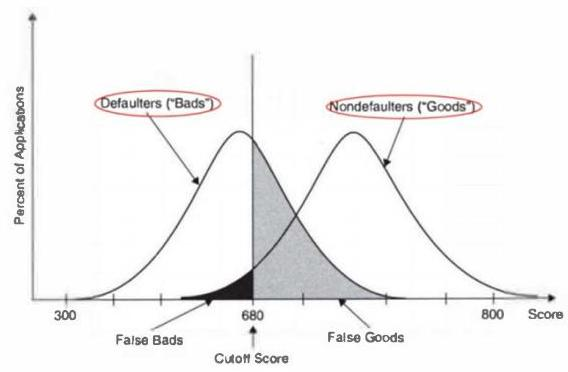
\includegraphics[width=0.4\textwidth]{images/019660e9-a588-71b6-ba51-02bd715bce7b_20_535_322_568_372_0.jpg}
\end{center}
\hspace*{3em} 

 设定 Cutoff Scores 的目的:避免放款给高风险客户，同时尽量不错过的低风险客户。

\item Scorecard Performance:

\begin{itemize}
\item 判断一些评分模型 Scoring Model 是否有效

\item 在衡量记分卡的性能时，传统上采用的验证技术是累积准确率曲线（CAP）及其汇总统计量，即准确率（AR）。When measuring a scorecard's performance， the validation technique traditionally employed is the cumulative accuracy profile (CAP) and its summary statistic， the accuracy ratio (AR).

\item 累计准确性曲线 (cumulative accuracy profile， CAP)
\begin{itemize}

\item 横坐标（horizontal axis ）为按得分从最高风险分值到最低风险分值排序的人群。

\item 纵坐标（vertical axis ）是根据银行记录得出的实际违约百分比。

\item 完美模型(perfect model)曲线:代表最完美的情况下，模型会识别出所有坏客户。此时， CAP 曲线是折现(由下图红色箭头组成)；

\item 随机模型(random model)曲线:代表模型对好坏客户毫无区分能力， CAP 曲线会是一条斜率为 45 度的线(下图率色箭头)；

\item 实际模型(actual model)曲线:代表实际模型的曲线，越接近完美曲线代表预测能力越强；越接近随机曲线，代表预测能力越弱。
\end{itemize}
\end{itemize}

\begin{center}
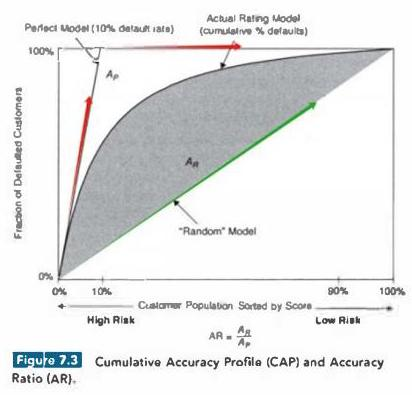
\includegraphics[width=0.3\textwidth]{images/019660e9-a588-71b6-ba51-02bd715bce7b_20_620_1731_412_395_0.jpg}
\end{center}
\hspace*{3em} 

\item 完美模型(perfect model)下的面积记为 \(\mathrm{{Ap}}\) ，而实际评分模型(actual rating model )下的面积记为 \({\mathrm{A}}_{\mathrm{R}}\)

\[
\text{ accuracy ratio }\left( \mathrm{{AR}}\right)  = \frac{{\mathrm{A}}_{\mathrm{R}}}{{\mathrm{A}}_{\mathrm{P}}}
\]

 AR 越接近 1 ，说明这个评分模型越准确。

\end{itemize}

\subsection{Country Risk CR-8}


【这是 24 年新增加的内容，和一级有很大的相似度，专有名词有变更、考纲要求稍微有些不同。如果一级学习的比较好，这里可以稍微看一下就行。

FRM 一级在 2020 年未改版之前， 关于 Country Risk 这个内容， 和现在 FRM 二级的这个知识点选用的是同一个人的同一篇文章， 只是版本不同而已 (FRM 二级比较新)。】

许多大公司在世界各地都有商业布局。虽然这些公司可能在一个国家注册成立， 但对它们来说， 评估它们在国外经营相关的风险是很重要的。这些风险统称为国家风险或国别风险(country risk)。

【本章节的逻辑: country risk 的来源成因 \(\rightarrow\) country risk 的衡量 (几个机构在做这个事情，但有缺陷) \(\rightarrow\) (抓主要矛盾) \(\rightarrow\) 衡量主权债务违约风险( 2 种手段) \(\rightarrow\) 主权信用评级 V.S 信用价差 \(\rightarrow\) 这两种手段各有优缺点】


\begin{itemize}

    \item 1. Evaluation of Risk

\begin{itemize}
\item Economic Growth Life Cycle 经济增长生命周期
\begin{itemize}

    \item 评估国家风险的一个重要考虑因素是一个国家将如何应对经济周期。 An important consideration in assessing country risk is how a country will respond to economic cycles.

\item 在经济衰退期间，发展中国家国内生产总值的下降幅度往往大于发达国家。During economic downturns， GDP in developing countries tends to decline more than GDP in developed countries.

\item 核心思想:在成熟市场，国家风险较低；在新兴市场，国家风险较高。 
\end{itemize}

\item - Political risk
\begin{itemize}


    \item 政治风险是指政府、政府决策或政府运作方式的变化对企业或投资的盈利能力产生重大影响的风险。Political risk is the risk that changes in governments， decisions made by governments， or the way governments operate will significantly affect the profitability of a business or an investment.


    \item 评估政治风险绝非易事。Assessing political risk is never easy.

    \begin{itemize}

        \item Democracies 民主制 or authoritarian 独裁制 governments

        \item Corruption 腐败

 \item Violence 暴力

 \item Nationalization 国有化 or expropriation 征用
\end{itemize}
\end{itemize}

\item Legal Risk
\begin{itemize}

    \item Legal risk is the risk of losses due to inadequacies or biases in a country' s legal system. Property rights and contract enforcement are important aspects of a legal system.

    \item 核心思想:法律体系是否健全有效 - 
\end{itemize}

 \item Economic Structure
 \begin{itemize}

    \item It is also important to assess the country's competitive advantages and the extent to which its economy is diversified.

    \item 过度依赖单一商品/服务的经济体风险较高，比如过度依赖石油、或旅游业等。

    \item 经济多样化在小型经济体中很难实现。
\end{itemize}
\end{itemize}

 \item 2. 国家风险的衡量

对于国家风险的衡量是否存在一个可靠的综合的风险度量 (比如， 求出一个国家的 VaR 或 ES)。有几个机构在做这个事情:

\begin{itemize}
\item Political Risk Service (PRS)

\begin{itemize}
\item Uses 22 measures of political， financial and economic risk to calculate its index. Individual companies can customize the PRS forecasting model to their own projects or exposures.
\end{itemize}

\item 媒体机构: provide country risk scores.
\begin{itemize}


\item Euromoney's score is based on a survey of 400 economist.


\item The Economist develops country risk scores internally based on currency risk， sovereign debt risk， and banking risk.
\end{itemize}

\item The World Bank

\begin{itemize}
\item Provides country risk data measuring corruption (腐败)， government effectiveness， political stability， regulatory quality， the rule of law， and accountability.
\end{itemize}

\item 要注意这么几个问题:
\begin{itemize}

    \item 1) 几个机构之间的评分无法进行比较。It is difficult to compare these services because they use different scoring methods and consider different attributes of country risk.

    \item 2) not every dimension of country risk is necessarily relevant to every individual or corporation.

    \item 3) the question of scaling (评分的尺度问题): 如果 \(\mathrm{A}\) 国家的得分是 \(\mathrm{B}\) 国的两倍，并不意味着 \(\mathrm{A}\) 国的风险是 \(\mathrm{B}\) 国的两倍。因此，国家的得分排序 (rankings of countries)比它们分数本身(their numerical scores)更有意义。
\end{itemize}
\end{itemize}

\item 3. Sovereign Credit Risk

\begin{itemize}
\item One measure of a country's risk is the risk it will default on its debt. There are two types of sovereign debt: the type issued in a foreign currency (such as the USD) and the type issued in the country's own currency.衡量一个国家的风险大小问题， 一个主要的代表就是看其政府债务的履约情况。即衡量其主权债务违约的风险。主权债务 (sovereign debt) 有两种类型: 以外币发行债务和以本国货币发行的债务。


\item Foreign Currency Defaults 外币违约

\begin{itemize}

    \item 以外币发行的债务

    \item 发行国无法通过简单地印更多的钱(print more money)来偿还债务。

    \item 违约是由金融、经济和政治问题共同造成的，这些问题在最初发放贷款时基本上是无法预见的。

    \item 举例来说， 美国政府可以通过印刷更多的美元来偿还以美元发行的债务 (被称为增加货币供应量，并可能导致通货膨胀)。然而，像阿根廷这样的国家在借入美元时就无法用印美元的方式来还钱。

    \item 例如:希腊债务危机:南美的有些国家在过去 200 年中多次违约。
\end{itemize}

\item Local Currency Defaults 本币违约
\begin{itemize}

    \item 一些国家对以本国货币发行的债务以及以外币计价的债务违约。

    \item 例如:巴西(1990 年)和俄罗斯(1998 年)的违约

    \item 穆迪的研究表明，这两类债务同时违约的国家越来越多。

    \item Reasons: 【既然很多国家可以印更多的钞票，为什么它们还会违约以本国货币计价的债务? 是小可爱吗? 不是】

 客观上:无法印钱(print money)

比如， 1971 年之前， 要有对应的黄金储备， 才能印对应的钱: 希腊债务危机 (2012 年)， 希腊没有印制欧元的权利。

 In the decades before 1971， currencies had to be backed by gold reserves.

 Members of the European Union use the euro as their domestic currency.

 Printing more money debases the currency and leads to inflation

 \item  主观上:印钱 (print money) 带来的危害更大

 一方面，印更多的钱会使货币贬值并导致通货膨胀。

 另一方面，印钞在短期内可能解决一部分问题，但长期看危害较大。
\end{itemize}
\item Impact of a Default
\begin{itemize}
    

    \item     The modern consequences of a default by a sovereign nation include:

    \item A loss of reputation along with an increased difficulty in raising funds for several years

    \item A lack of investors willing to buy the debt and equity of corporations based in the country

    \item An economic downturn (经济衰退)

\item Political instability as the population loses faith in its leaders

\item A default has a negative impact on GDP growth， has a negative impact on the country's credit rating for many years， can hurt exports， and can make the banking system of the defaulting country more vulnerable. 【违约对 GDP 增长有负面影响， 对该国的信用评级有多年的负面影响， 可能损害出口，并可能使违约国的银行系统更加脆弱。】
\end{itemize}

\item Factors Determining Sovereign Default Risk

【政府违约的原因与个人和企业违约的原因相似:在经济繁荣时借贷超过其收入；在经济衰退时，无法履行债务义务。】

 债务程度 Degree of indebtedness: 看一个主权实体欠多少债，不仅是对外债务， 还有对内的债务。

评级机构会使用 government debt-to-GDP ratio 来衡量国家的债务水平。

Table 8.3 Debt as \% of Gross Domestic Product in 2020

\begin{center}
\adjustbox{max width=\textwidth}{
\begin{tabular}{|c|c|c|}
\hline
Country & In 2010 & In 2020 \\
\cline{1-3}
Venezuela & 25.00\% & 304.13\% \\
\cline{1-3}
Japan & 205.69\% & 254.13\% \\
\cline{1-3}
Greece & 147.49\% & 211.21\% \\
\cline{1-3}
Italy & 119.20\% & 155.82\% \\
\cline{1-3}
Portugal & 100.21\% & 135.19\% \\
\cline{1-3}
United States & 95.14\% & 133.92\% \\
\cline{1-3}
Spain & 60.52\% & 119.92\% \\
\cline{1-3}
Cyprus & 56.43\% & 119.14\% \\
\cline{1-3}
Canada & 81.22\% & 117.46\% \\
\cline{1-3}
France & 85.26\% & 115.08\% \\
\cline{1-3}
Belgium & 100.27\% & 114.14\% \\
\cline{1-3}
Montenegro & 45.01\% & 107.15\% \\
\cline{1-3}
United Kingdom & 74.27\% & 104.47\% \\
\cline{1-3}
Mauritius & 57.15\% & 99.91\% \\
\cline{1-3}
Brazil & 62.43\% & 98.09\% \\
\cline{1-3}
Egypt & 69.59\% & 89.84\% \\
\cline{1-3}
India & 66.40\% & 89.61\% \\
\cline{1-3}
El Salvador & 60.04\% & 89.17\% \\
\cline{1-3}
Croatia & 57.68\% & 88.74\% \\
\cline{1-3}
Saint Vincent and the Grenadines & 65.45\% & 85.00\% \\
\cline{1-3}
\hline
\end{tabular}
}
\end{center}

Source: IMF


    \item 养老金／社会服务承诺Pensions/SocialService Commitments: 社会福利好的国家， 可能应具有更高的违约风险。
    \item 政府收入／流入Revenues/Inflows to government: 政府收入通常来自税收， 这取决于税法和税基。较大的税基可以增加潜在税收收入， 从而用于偿还债务。
    \item 收入的稳定性Stability of revenues: 债务必须在好坏时期都要偿还。因此， 收入流更稳定的国家违约风险较低。
    \item 政治风险Political risk: 专制政权可能比民主政权更容易违约。此外，中央银行的独立性和权力也会影响违约风险。
    \item Implicit backing隐性支持from other entities
\end{itemize}

\item 4. Sovereign Credit Ratings

【评级机构通常提供本币评级(local currency ratings)和外币评级(foreign currency ratings)。】

\begin{itemize}
    \item 本币评级： 对一个国家本币债务违约的可能性的意见。
    \item 外币评级： 对其外币债务的违约可能性的意见。
    \item 本币评级和外币评级的差异主要基于一个国家的货币政策独立性(monetary policy independence)。
    \begin{itemize}
        \item 失去货币政策独立性的国家（例如欧盟国家）其本币和外币评级将趋于
        一致。
        \item  拥有浮动汇率制度并可以通过稳健的国内市场进行借款的国家，其本币
        和外币评级差异最大， 通常本币评级较高。
    \end{itemize}
    \item 评级机构的两种方法：
    \begin{itemize}
        \item 上调法(Notch-up approach)
        \begin{itemize}
            \item 外币评级是主权违约风险的关键指标，本币评级在此基础上
            进行上调。
        \end{itemize}
        \item 下调法(Notch-down approach) :
        \begin{itemize}
            \item 本币评级是主权违约风险的关键指标，外币评级在此基础上
            进行下调。
        \end{itemize}
    \end{itemize}
    \item Shortcomings of the sovereign rating systems:
    \begin{itemize}
        \item Ratings are biased upward.
        \item  Herd behavior羊群行为当一个评级机构上调或下调一个国家的评级时，
        其他评级机构往往会跟随。
        \item  Too little， too late。评级变化不及时。
        \item ViciousC ycle恶性循环
        \item  Ratings failures评级失败
    \end{itemize}
    
\end{itemize}


\item 5. 衡量主权债务风险

【评级机构的主权债务评级可以在一定程度上衡昼主权债务风险，有缺陷。可以
采用更加基于市场的衡量方式： Sovereign Default Spread、CDS spread】

\begin{itemize}
    \item (1) Sovereign Default Spread主权违约利差
    \begin{itemize}
        \item The credit spread for sovereign debt in a given currency is the excess
        interest paid over the risk-free rate in that currency.
        \item 这一利差反映了市场对该国的信用风险。
        \item  例如，2022年7月1日， 巴西政府发行了一笔10年期美元计价债券，市场
利率为6\%。与此同时， 美国政府10年期国债的利率为3.02\%。
    \begin{itemize}
    \item  Sovereign Default Spread=6\% -3.02\% = 2.98\%)
    \end{itemize}
\item  主权违约利差可以在一定程度上反映一国偿还债务能力
\item  主权违约利差与评级之间存在着很强的相关性。

\begin{center}
    \textbf{Default Spreads on US \$D enominated Bonds-Emerging Markets in July 2022}
    \end{center}
    
    \begin{center}
        {\renewcommand{\arraystretch}{1.5}
        \begin{tabular}{|l|c|c|c|c|}
        \hline
        \textbf{Country} & \textbf{Moody's Rating} & \textbf{\$ 10-year Bond Rate} & \textbf{US T.Bond Rate} & \textbf{Default Spread} \\
        \hline
        Brazil & Ba2 & 6.19\% & 3.02\% & 3.17\% \\
        \hline
        Chile & A1 & 4.33\% & 3.02\% & 1.31\% \\
        \hline
        Colombia & Baa2 & 5.58\% & 3.02\% & 2.56\% \\
        \hline
        Indonesia & Baa2 & 4.38\% & 3.02\% & 1.36\% \\
        \hline
        Mexico & Baa1 & 5.07\% & 3.02\% & 2.05\% \\
        \hline
        Peru & Baa1 & 4.76\% & 3.02\% & 1.74\% \\
        \hline
        Turkey & B2 & 10.92\% & 3.02\% & 7.90\% \\
        \hline
        \end{tabular}}
    \end{center}

\item 比较：
\begin{center}
    \begin{tabular}{|c|c|c|}
    \hline
    & \textbf{Sovereign Default Spread} & \textbf{Sovereign Credit Ratings} \\
    \hline
    相同点 & \multicolumn{2}{c|}{都可以反映一国偿还债务的能力} \\
    \hline
    \multirow{3}{*}{不同点} & more granular 颗粒度 than ratings & \multirow{3}{*}{评级较稳定（评级稳定性是评级机构的目标之一）} \\
    \cline{2-2}
    & 比评级更快地适应新信息 & \\
    \cline{2-2}
    & 不稳定 & \\
    \hline
    \end{tabular}
    \end{center}
    \end{itemize}


    \item (2) CDS spread (credit default swap spread)
    \begin{itemize}
        \item CDS spread也可以作为主权债务的违约风险
        \item 在这里CDS其参考实体是主权国家政府的债务， 而不是公司债务。例如， 如
        果购买了秘鲁政府债券的CDS， 那么秘鲁政府就是这个CDS合同中的参考实
        体。
        \item 如果参考实体（某个主权政府）风险大，CDS spread大；
        \item 如果参考实体（某个主权政府）风险小， CDSspread小；
        \item  优点：
        \begin{itemize}
            \item  CDS利差基于市场交易， 反映市场看法， 可以比信用评级更好地预测主
        权风险

    \end{itemize}
        \item  缺点：
        \begin{itemize}
            \item  首先， CDS利差反映了包括信用风险、市场风险和流动性风险在内的多
        种风险， 单纯依靠CDS利差评估信用风险可能会高估风险。
        \item   其次， CDS市场常常存在流动性不足的问题， 这可能扭曲其价格。
    \end{itemize}
\end{itemize}

\end{itemize}




\end{itemize}
